\section{System Design}

\subsection{Design Paradigm}

\subsection{Data-flow diagram}
\begin{figure}[H]
    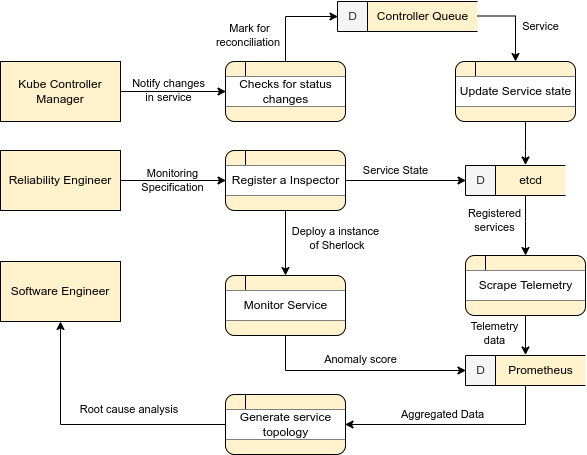
\includegraphics[width=14cm]{assets/system-design/data-flow.png}
    \caption{Data-flow diagram (self-composed))}
    \label{fig:data-flow}
\end{figure}

\subsection{Sequence Diagram}

\begin{figure}[H]
    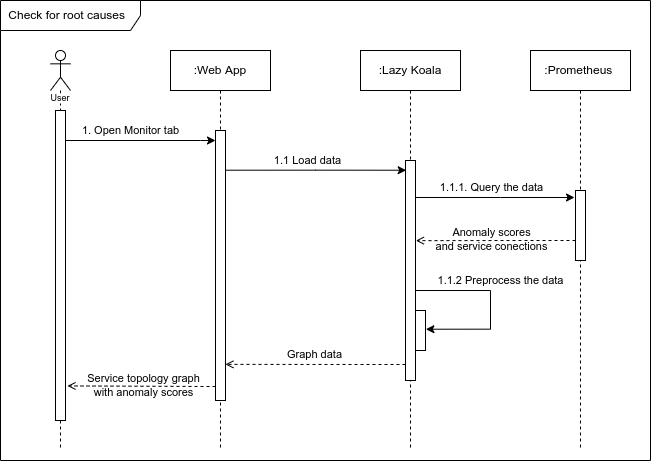
\includegraphics[width=14cm]{assets/system-design/sequence-diagram-1.png}
    \caption{Sequence Diagram for checking Check for root cause (self-composed))}
\end{figure}

\begin{figure}[H]
    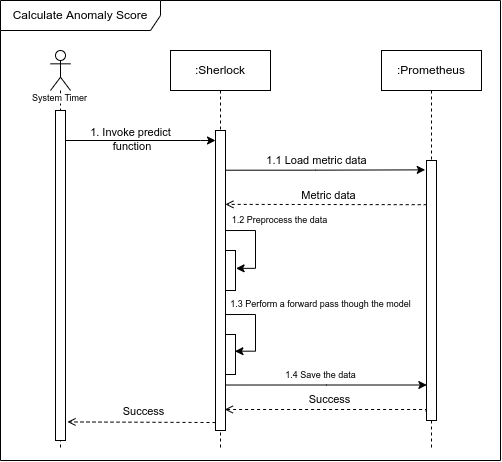
\includegraphics[width=14cm]{assets/system-design/sequence-diagram-2.png}
    \caption{Sequence Diagram for calculating anomaly score (self-composed))}
\end{figure}

\subsection{UI Mockups}

\begin{figure}[H]
    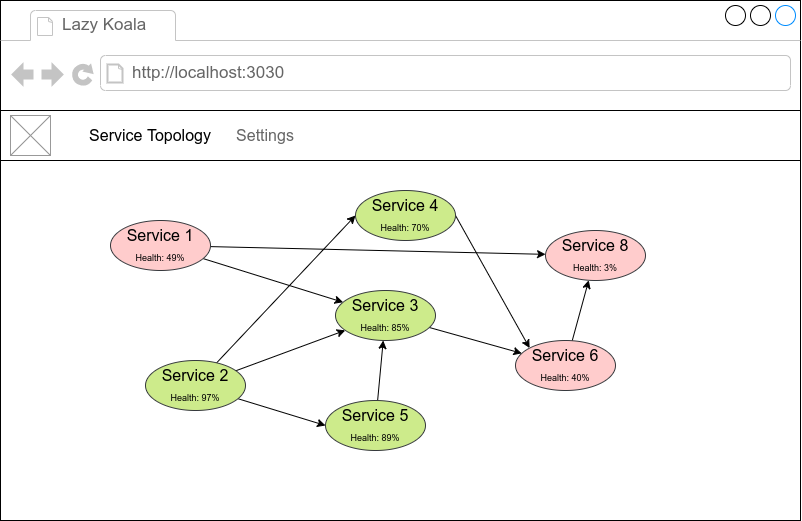
\includegraphics[width=14cm]{assets/system-design/ui-home.png}
    \caption{UI Mockup - Service Topology  (self-composed))}
\end{figure}

\begin{figure}[H]
    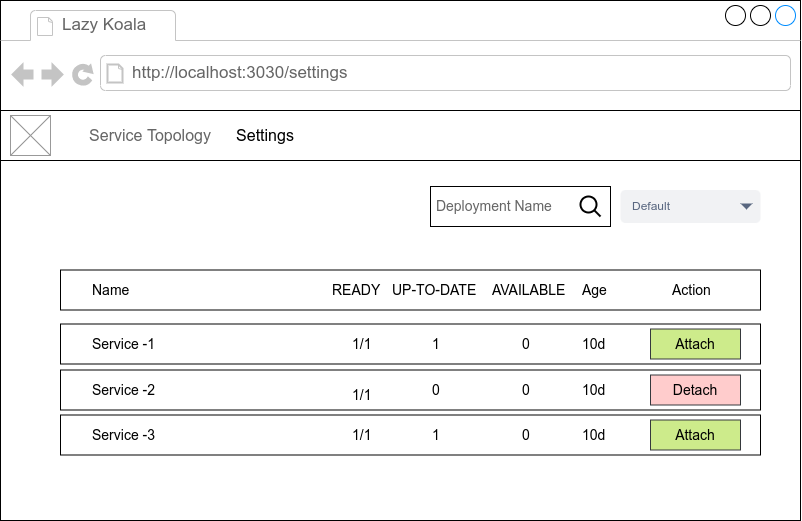
\includegraphics[width=14cm]{assets/system-design/ui-settings.png}
    \caption{UI Mockup - Settings (self-composed))}
\end{figure}